\chapter{Solução}

\section{Solução de Software}

O subsistema de software será dividido em dois Web Apps, o web app para o cliente e o web app para o vendedor. Esses dois webapps farão comunicação com um webservice, construído pela equipe de software.

	O web app do vendedor permite a a manutenção do estoque de picolés. Ele poderá cadastrar diferentes sabores em diferentes quantidades, a qualquer momento. 
%     Além disso o vendedor também poderá enviar uma notificação, compartilhando sua localização com todos os clientes próximos. Eles, então, poderão traçar uma rota para comprar o picolé. 
    Outra funcionalidade, é de ler relatórios sobre vendas e formas de pagamento.
    
    O web app do cliente terá a função de compra. O cliente em posse do app pode selecionar o vendedor e sabor do picolé que deseja comprar. Após determinado a quantidade dos sabores desejado o cliente irá inserir o número do cartão de crédito e efetuar a compra. Após confirmação do pagamento, o aplicativo libera um botão, o qual será responsável pela liberação do picolé. Com o botão liberado, o cliente se dirige até o carrinho em questão no momento que desejar e pressiona o botão, com isso, os picolés comprados são liberados e o usuário pode retirar seu pedido. Além disso, o cliente poderá traçar uma rota para o vendedor que escolher.

\begin{itemize}
	\item Formas de pagamento:
    \begin{itemize}
		\item \textbf{Dinheiro:} Somente o vendedor tem acesso a esta opção. Evita que alguém tenha que digitar o número do cartão para fazer o pedido, caso esteja sem o celular ou sem o app, ao mesmo tempo que ainda força a venda a ser feita pelo app, atualizando o estoque.

        \item \textbf{Cartão:} Integração com um gateway de pagamento, para possibilitar o pagamento em cartão. O app não armazenará os dados de cartão do cliente em hipótese alguma.
  	\end{itemize}

	\item Integração com outros serviços:
  	\begin{itemize}
    	\item \textbf{Localização:} Vendedor deve habilitar o uso da localização
    	\item \textbf{Maps:} Cliente pode ver o vendedor mais próximo e traçar rota até ele.
  	\end{itemize}

	\item Relatórios:
  	\begin{itemize}
        \item Quantidade de vendas: por período/por sabor
        \item Variação da temperatura interna do refrigerador (sensor de temperatura)
        \item Proporção de vendas por modo de pagamento
  	\end{itemize}
\end{itemize}


\section{Solução de Eletrônica}

\subsection{Sistemas Eletrônicos}

A parte eletrônica da máquina de vendas de picolé poderá ser dividido nos seguintes sistemas:

\subsubsection{Sistema GPS e Segurança}

A máquina de vendas terá um sistema de segurança utilizando-se um sistema de posicionamento global (GPS). O módulo GPS utilizado terá um chip GY-NEO6MV2 o qual é um módulo da família de GPS u-blox stand-alone de alta performance de posicionamento. Estes receptores são rentáveis e oferecem diversas opções de conectividade em um tamanho de 16 x 12,2 x 2,4 mm. Sua arquitetura, compacta de baixa tensão de operação (3.3 V) e memória, tornam os módulos NEO-6 ideais para dispositivos móveis operados com bateria e restrições de custo e espaço \cite{mq1}, que é o caso da máquina de vendas. A seguir, a figura \ref{fig:GPS} demonstra o módulo escolhido:

\begin{figure}[H]
	\centering
    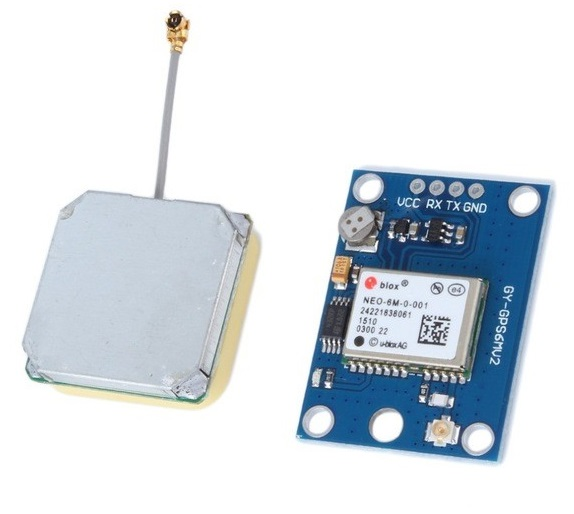
\includegraphics[width=0.5\textwidth]{figuras/modulo_gps}
    \caption{Módulo GPS da família u-blox}
    \label{fig:GPS}
\end{figure}

\subsubsection{Sistema de Som e Alarme}

Como haverá um sistema de segurança integrado ao projeto, será necessário emitir um aviso caso a máquina de vendas seja violado ou removido do local designado pelo vendedor. Além disso, haverá um assistente com voz automática para receber um cliente próximo à máquina de vendas e, quando não houver nenhuma pessoa por perto, o sistema emitirá uma propaganda do produto. O sistema de som será responsável por atender os clientes quando estes se aproximam, fazer propaganda e alarmar em caso de violação.

O sistema de som será composto por um módulo amplificador com o circuito integrado TDA8571, o qual é um amplificador dedicado capaz de oferecer 40 W para até 4 alto falantes de 4 ohms cada, totalizando 160 W no total. Possui tensão de alimentação de 12 V, o qual é a fornecida pela bateria. Possui poucos componentes externos, o que torna o circuito pequeno, além de possuir proteção contra curto-circuitos, descarga eletrostática e inversão de polaridade \cite{mq2}. O volume do som será dimensionado conforme a disponibilidade energética da máquina de vendas.

\subsubsection{Sistema de sensoriamento}

O projeto exige duas medidas para garantir seu bom funcionamento: a temperatura interna do recipiente dos picolés em resfriamento e um detector de presença para atender um possível cliente e para o sistema de alarme. 

	Para a medida de temperatura, será utilizado o sensor DS18B20 (que opera de 3.3 a 5 volts) à prova d'água fabricado pela Maxim Integrated, o qual é ideal para medidas em temperaturas na faixa de -10ºC a 85ºC com precisão de 0.5ºC, obtendo uma faixa de operação ainda maior. O sensor já possui uma saída digital, a qual pode ser transmitida diretamente para o Raspberry PI 3, realizando o controle de acionamento do sistema de refrigeração. A figura \ref{fig:sensor_temperatura} ilustra o sensor.
    
\begin{figure}[H]
	\centering
    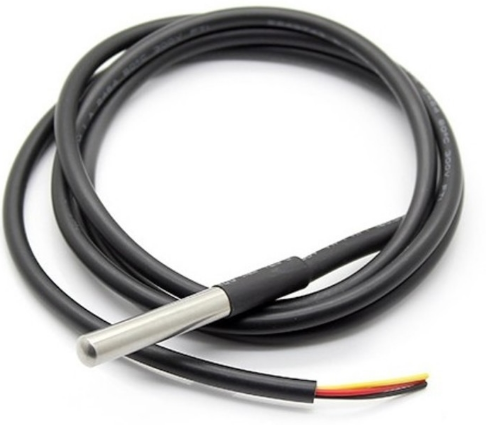
\includegraphics[width=0.5\textwidth]{figuras/sensor_temperatura}
    \caption{Sensor de temperatura}
    \label{fig:sensor_temperatura}
\end{figure}

O instrumento de sensoriamento de presença é o sensor ultrassônico de distância HC-SR04 (que opera a 5 volts), o qual será utilizado para detectar clientes nos quatro lados do recipiente de vendas (utilizando assim, quatro sensores) e para detectar a liberação de um picolé. O mesmo possui um alcance máximo de 4 metros e mínimo de 2 centímetros, sendo ideal para a detecção de usuários que se aproximam da máquina de vendas \cite{mq3}. A figura \ref{fig:sensor_presenca} ilustra o sensor.

\begin{figure}[H]
	\centering
    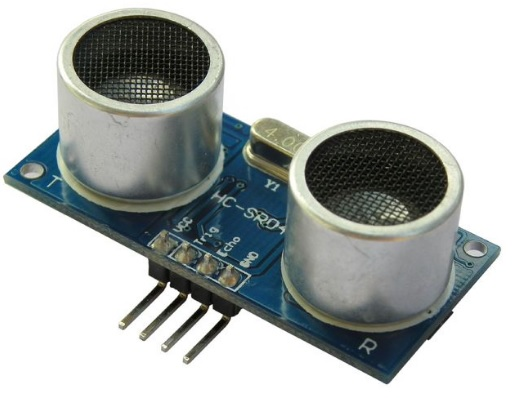
\includegraphics[width=0.4\textwidth]{figuras/sensor_presenca}
    \caption{Sensor de presença}
    \label{fig:sensor_presenca}
\end{figure}

\subsubsection{Sistema dos servomotores}
Os picolés serão entregues por meio de um sistemas de molas similar a de máquinas de venda. Um picolé situado no meio de uma mola faz um movimento linear quando este se rotaciona, como ilustra a imagem \ref{fig:sistema_molas} a seguir:

\begin{figure}[H]
	\centering
    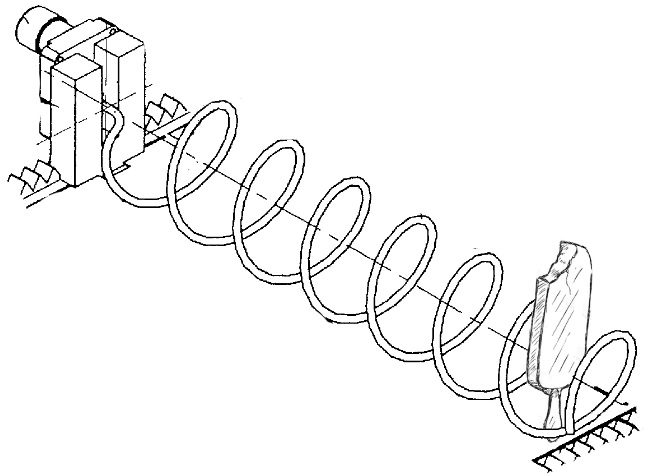
\includegraphics[width=0.8\textwidth]{figuras/sistema_molas}
    \caption{Sistema de molas capaz de movimentar os picolés}
    \label{fig:sistema_molas}
\end{figure}

Logo, será necessário inserir um motor no final de cada mola e fazer o controle do giro para os picolés caírem conforme o pedido do cliente. Para isso, o tipo de motor escolhido foi o \textbf{servomotor}, já que possui torque suficiente para movimentar a longa fileira de picolés situados na mola com uma precisão de uma volta (360\degree por venda). Além disso, seu controle é feito por meio de apenas um fio, em contraste ao motor de passos que é necessário utilizar um driver que controla diversos fios para cada.

\subsubsection{Sistema do Acionamento do Compressor}

A refrigeração do recipiente vai ser feita por meio de um compressor. Mantê-lo ligado o tempo todo não é viável devido à limitação da demanda energética. Para isso, será feito um controle de acionamento do compressor de acordo com os dados enviados pelo sensor de temperatura. Para ligar e desligar o compressor, será utilizado um módulo relé JQC-3F. O relé é um componente eletro mecânico capaz de realizar a função de uma espécie de chave selecionadora. Por meio dela, é possível fazer o acionamento de sistemas de alta potência com um controlador (i.e. Raspberry Pi) sem danificá-lo e puxar muita corrente.

\subsubsection{Sistema de interface visual}

A ideia central da máquina de vendas é a sua capacidade de realizar vendas de picolé sem um vendedor presente pelo aplicativo de celular. Portanto, convém utilizar um sistema visual na qual poderá mostrar informações ao usuário tais como:

\begin{itemize}
  \item O estoque dos sabores dos picolés;
  \item Um rápido tutorial de como obter e utilizar o aplicativo;
  \item Caso o picolé seja vendido, informar ao usuário sua retirada;
  \item Fazer propaganda do produto.
\end{itemize}

Para isso, haverá uma tela LCD embutido no máquina de vendas de fácil visualização para os clientes.

\subsection{Integração de todos os sistemas eletrônicos}

O controlador escolhido para integrar todos os sistemas será o Raspberry Pi 3, o qual é possui um computador que possui um processador ARM de 1.2 GHz 64 bit, 1 Gb de RAM e bluetooth. Ficou popular por ser intuitivo de utilizar, o que fez com que seja utilizado no mundo inteiro em diversos projetos eletrônicos. Possui capacidade de embutir um sistema operacional como o Linux, o que pode tornar o sistema mais estável e com menos memória de uso. Sua escolha se justifica pelo fato de conter todos os requisitos exigidos para cada sistema, tais como:

\begin{itemize}
  \item Possui entradas e saídas digitais as quais podem ser usadas para controle dos sistemas GPS e controle dos motores e controle do sensoriamento;
  \item Possui saída de áudio para o sistema de som;
  \item Possui saída de vídeo para o sistema de interface com o usuário.
\end{itemize}

Além disso, depois de projetado e testado cada sistema, será confeccionado no final uma \textbf{placa de circuito impresso (PCI)} para conter todos os circuitos de forma compacta, já que o espaço do projeto é limitado.

\subsection{Integração entre Software e Hardware}
A comunicação entre software e hardware será feita via internet e, para isso, será utilizado o módulo GSM GPRS SIM900 fabricado pela SIMCom. O módulo interligado à Raspberry PI 3 utilizará um cartão SIM para conexão com a internet e, dessa forma, a comunicação com o sistema de software será estabelecida.

\begin{figure}[H]
	\centering
    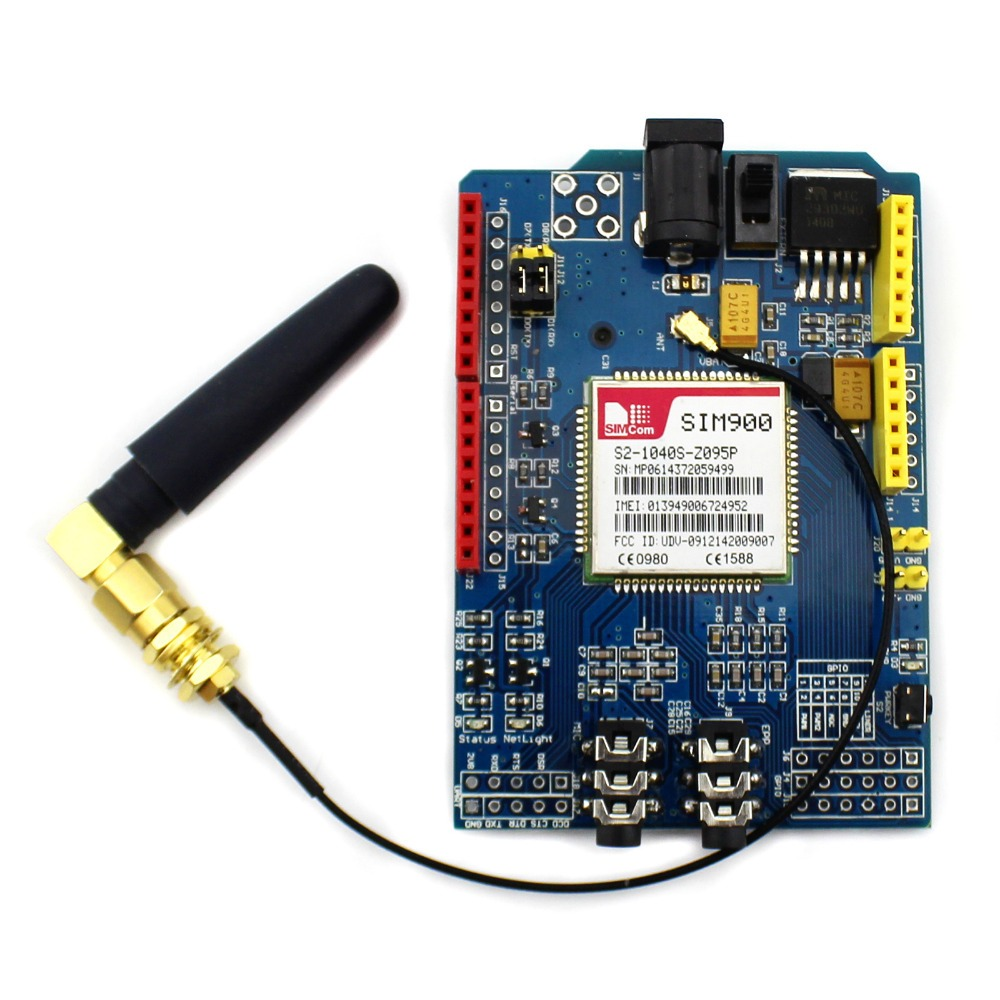
\includegraphics[width=0.6\textwidth]{figuras/modulo_gprs}
    \caption{Módulo GPRS SIM900 (SIMCom)}
    \label{fig:modulo_gprs}
\end{figure}

\section{Solução de Estrutura}
Como solução para a estrutura foram levantadas várias possibilidades de produtos para realizar a venda dos picolés, afim de escolher um conjunto que atenda às necessidades da indústria de picolés. À principio as opções eram:

\begin{itemize}
\item Triciclo com compartimento dianteiro
\item Triciclo com compartimento traseiro
\item Máquina de venda estática
\end{itemize} 

\begin{figure}[H]
	\centering
    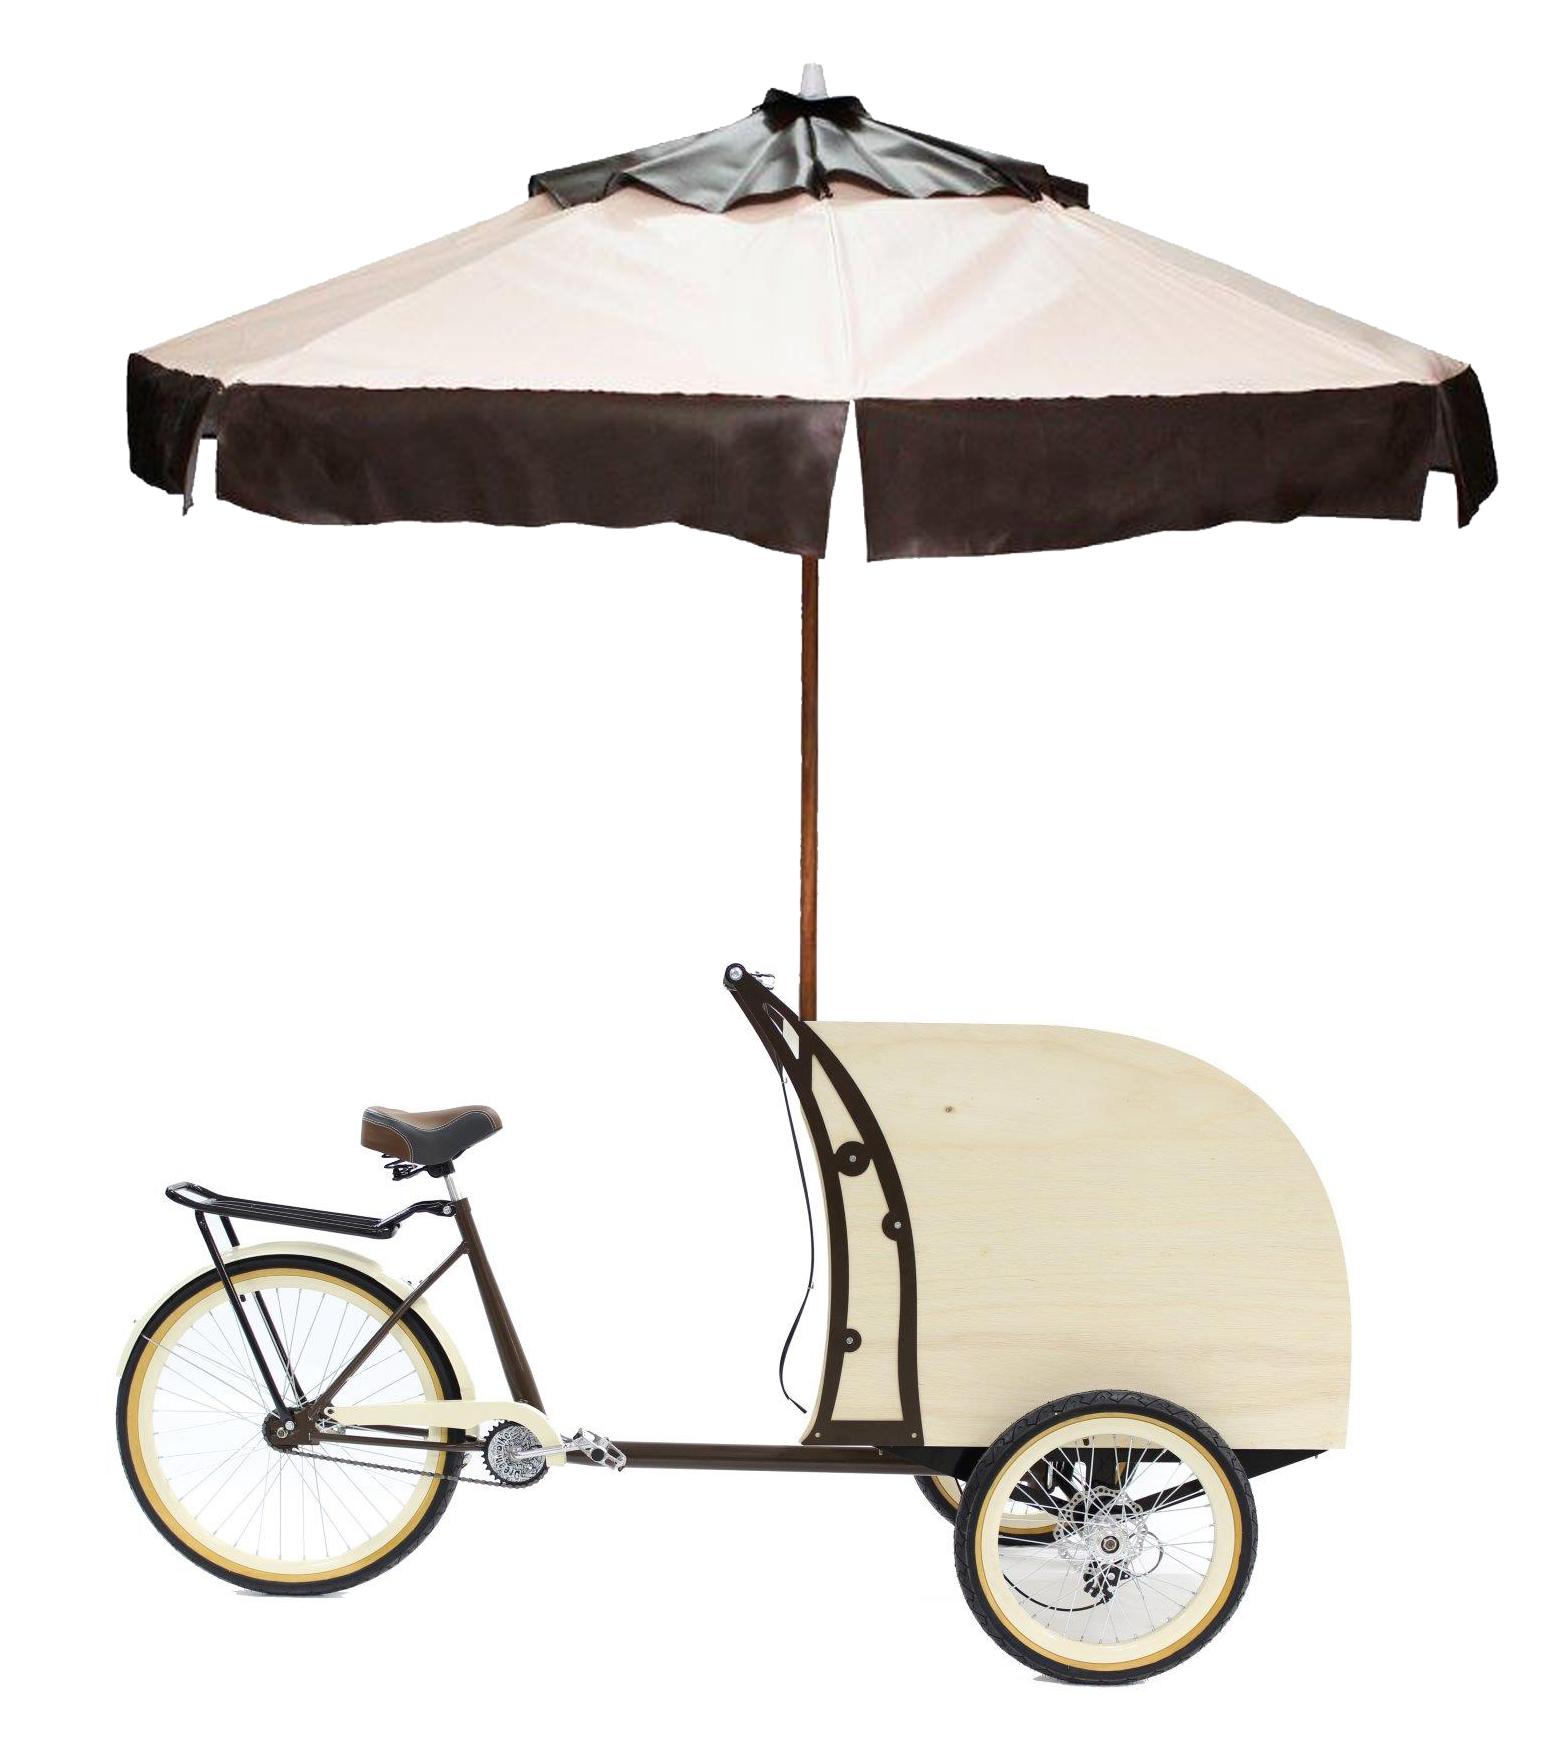
\includegraphics[width=0.6\textwidth]{figuras/exemplo2}
    \caption{Triciclo com Compartimento Dianteiro}
    \label{fig:exemplo2}
\end{figure}

\begin{figure}[H]
	\centering
    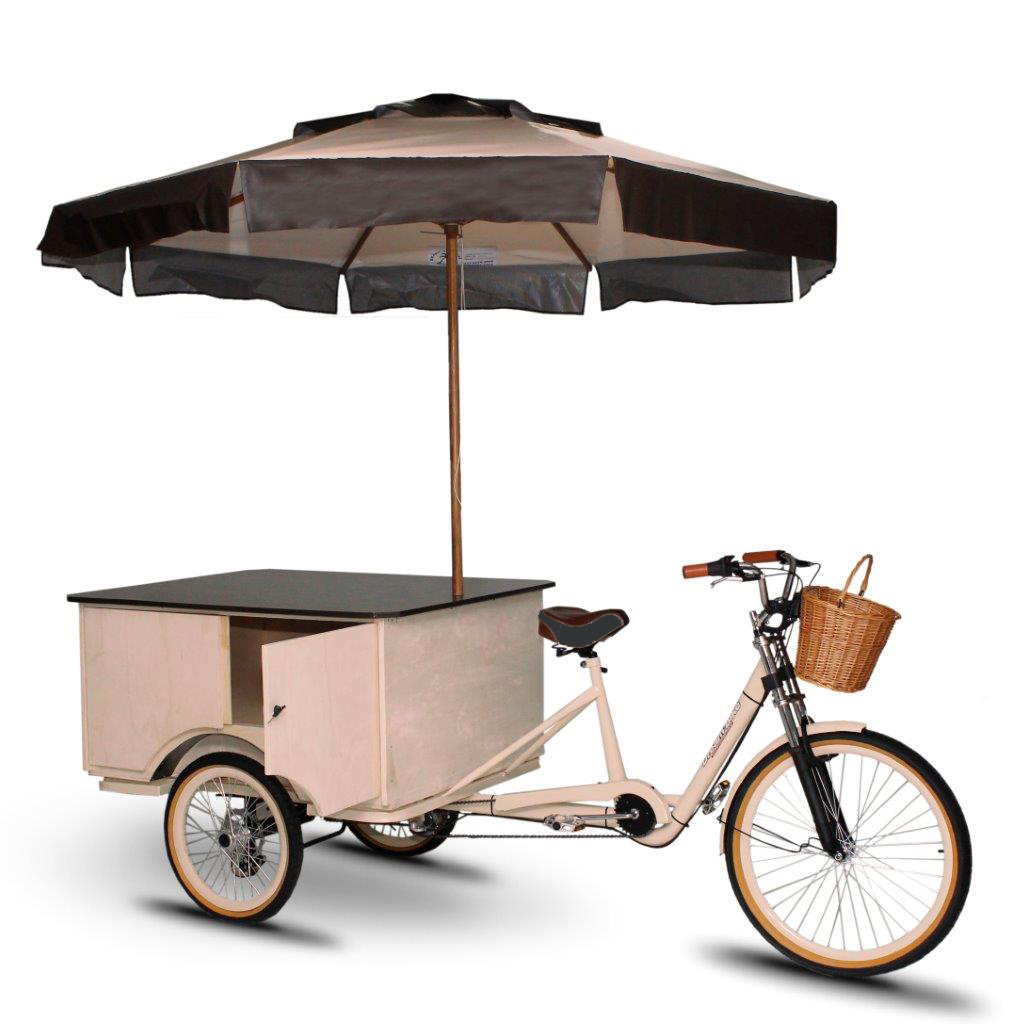
\includegraphics[width=0.6\textwidth]{figuras/exemplo}
    \caption{Triciclo com Compartimento Traseiro}
    \label{fig:exemplo}
\end{figure}

\begin{figure}[H]
	\centering
    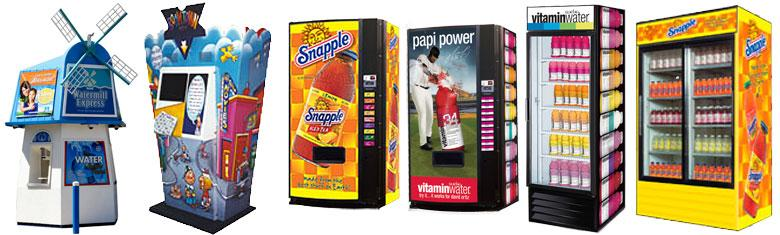
\includegraphics[width=0.6\textwidth]{figuras/machinewrapsheader}
    \caption{Vending Machines}
    \label{fig:machinewrapsheader}
\end{figure}

Após consultoria com a empresa de sorvetes Saborizze, não se tornou viável a utilização de triciclos no transporte da máquina de vendas automáticas devido a necessidade de um funcionário da empresa contratado apenas para conduzir o triciclo. Vendo isso, como solução de projeto de acordo com a aplicabilidade no mercado, foi escolhido como estrutura de projeto uma máquina de venda automática (\textit{vending machine}) que pode ser carregada por carro de transporte até o ponto de interesse pra ser realizada a venda dos picolés.

 As estruturas que compõe a máquina de venda se dividem nos seguintes tópicos:
 
 \begin{itemize}
\item Estrutura de suporte das placas solares



\item Mecanismos para venda automatizada de picolé



\item Compartimentos da máquina de vendas

A máquina de vendas devera possuir três compartimentos principais: compartimento para baterias e compressor, compartimento do freezer com isolamento térmico e compartimento para o componentes eletrônicos. 

\item Carrinho para o transporte da máquina de vendas

	Será montada uma estrutura para facilitar o transporte da máquina de vendas. Foi optado por uma estrutura simples e que pudesse ser acoplada à máquina durante seu transporte e depois desacoplada para assim poder ser reutilizada no transporte de outra máquina de vendas. 
	Para a montagem da estrutura de transporte da máquina, será feita a adaptação em uma estrutura já pronta mostrada na imagem abaixo:
    
   \begin{figure}[H]
	\centering
    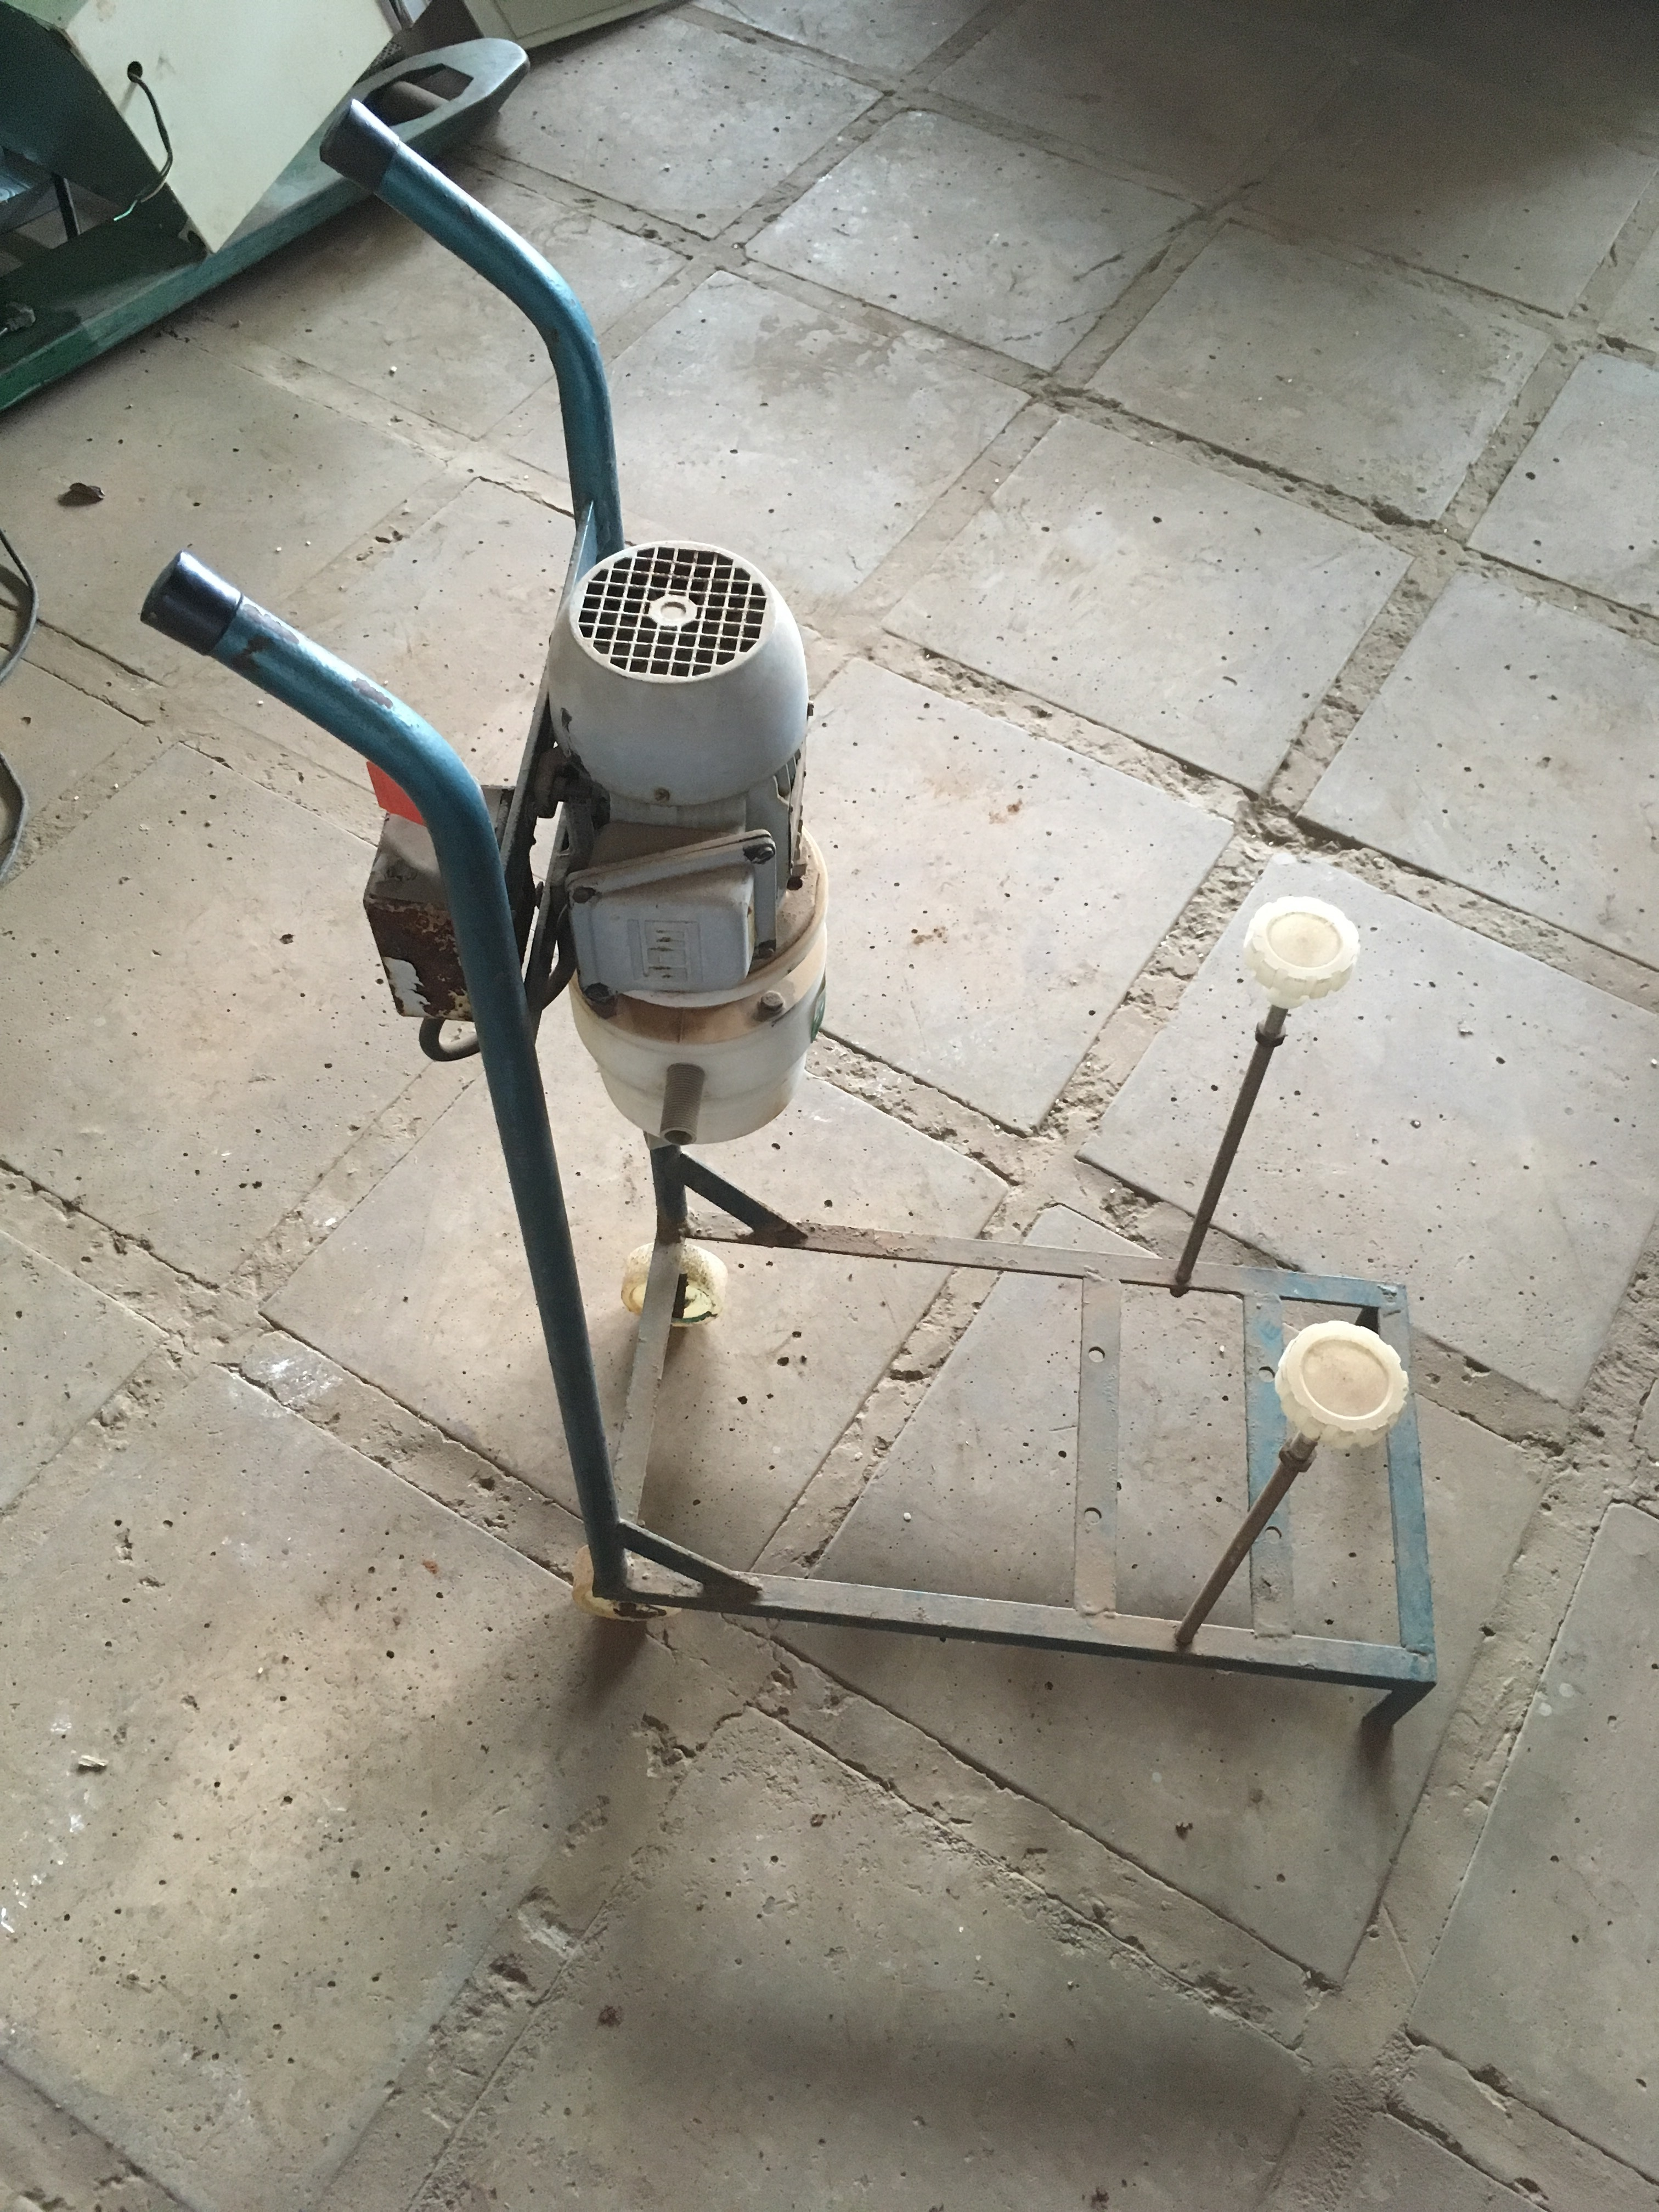
\includegraphics[width=0.4\textwidth]{figuras/mecanismodetransporte}
    \caption{Estrutura base para o transporte da máquina de vendas}
    \label{fig:mecanismodetransporte}
\end{figure}

\end{itemize} 

\subsection{Compartimentos}


\section{Solução de Energia}

\subsection{Refrigeração}
Atendendo aos requisitos definidos para o projeto, o recipiente no qual os picolés são armazenados deverá manter-se refrigerado durante o período de venda. O processo de refrigeração consiste em retirar calor de uma corpo ou espaço para reduzir sua temperatura e transferir esse calor para outro corpo ou espaço \cite{campos2010refrigeraccao}. Portanto, a partir da análise das características da demanda de refrigeração, custos limitados e o tempo hábil para a construção e integração do produto em questão, encontrou-se duas opções de resfriamento:

\begin{itemize}
\item Células de Peltier;
\end{itemize}

\begin{itemize}
\item Compressor;
\end{itemize}


O módulo de Peltier é a maneira mais prática de se utilizar o efeito peltier em larga escala, e consiste em um arranjo de pequenos blocos de \textit{telureto de bismuto - $Bi_{2}Te_{3}$} dopados tipo N e tipo P montados alternamente e eletricamente em série entre duas placas de cerâmica com alta condutividade térmica.Os semicondutores utilizados possuem altos coeficientes de Seebeck e podem ser tipo N $(\alpha \leq 0)$ e tipo P $(\alpha \geq 0)$  \cite{campos2010refrigeraccao}.

A utilização dos módulos de peltier tem as seguintes vantagens:

-Não utiliza partes mecânicas móveis para refrigeração;

-Aquece e resfria dependendo apenas da polaridade da alimentação;

-Dispensa o uso de gases refrigerantes, tecnologia 100 por cento estado sólido;

-Funcionam em qualquer orientação com/sem gravidade diferente dos refrigeradores baseados em compressores.


O resfriamento utilizando compressores ocorre por meio da compressão mecânica de vapor de um fluido refrigerante. Fluido refrigerante é uma substância que, ao circular dentro de um circuito fechado, é capaz de retirar calor de um meio enquanto se vaporiza a baixa pressão \cite{teixeiraconcepccao}.

Ao se optar pelo resfriamento por compressão tem-se as seguintes vantagens:

-Baixo consumo;

-Maior Eficiência;

Outra opção a ser utilizada no projeto é o resfriamento por meio de compressor, uma vez que o consumo da célula de peltier é extremamente alto, 70W para a placa de 40x40x4 milímetros. Para resfriar o recipiente seriam necessários entre 7 a 10 módulos, o que necessitaria uma fonte de 490W a 700W e um inversor. A fonte de fornecimento escolhida foi placas fotovoltaicas e para conseguir manter esse fornecimento seria necessário uma área para absorção de energia solar muito maior do que seria possível instalar no carrinho de picolé. 


Para o dimensionamento do compressor, é necessário calcular a potência necessária para fazer o fluido refrigerante circular pela serpentina. Essa potência foi encontrada a
partir da formulação:

\begin{math} W_{c} = m_{f} * (h_{2} - h_{1})  \end{math}

Onde:

$W_{c}$ é a potência teórica do compressor (kJ/h);

$m_{f}$ é o fluxo de massa refrigerante (kg/h);

$h_{2}$ é a entalpia no inicio da compressão (kJ/kg);

$h_{1}$ é a entalpia no final da compressão (kJ/kg);


\subsection{Alimentação}
	As fontes de energia que serão utilizadas para alimentar o sistema de refrigeração da máquina de picolé são painéis fotovoltaicos e baterias. O painel solar será dimensionado levando em conta a demanda energética a qual a mesma precisará suprir para manter o banco de baterias em condições de manter o refrigerador em operação durante o período solicitado, bem como os outros equipamentos consumidores e referentes às outras áreas.
    
\begin{itemize}
\item Bateria
\end{itemize}
	  
      A tomada de decisão para escolha de uma bateria deve considerar a tensão e a corrente.(MAGALHÃES,211). O cálculo de autonomia de uma bateria necessita de diversos dados. Existem 3 parâmetros os quais são considerados os principais para a a escolha de uma bateria: curva de descarga, capacidade de armazenamento e capacidade de descarga (MEGGLIAR,2006). A curva de descarga é a relação do decaimento da tensão ao longo do consumo da capacidade nominal. A capacidade da bateria quantifica o tempo para que ocorra uma descarga total, medido em Ah (Ampér hora). A capacidade de descarga é a quantificação da entrega de carga sem que ocorram danos à bateria.
      As baterias de chumbo-ácido são muito utilizadas em sistemas onde a há correntes  elevadas, como motores de arranque e máquinas elétricas. É composta por Chumbo e Ácido Sulfúrico em concentrações calculadas que variam de 27 à 37 por cento(ANDRADE,2005), podendo ser seladas ou não, possuindo vida útil de até 4 anos, apresentando assim uma boa relação de custo-benefício.
            
\begin{itemize}
\item Painel Fotovoltáico
\end{itemize}

		A tomada de decisão para escolha de um painel fotovoltáico deve considerar à demanda energética dos sistemas os quais serão alimentados, no caso da máquina de vendas especificamente, deverá carregar a bateria que alimentará o compressor, e deixa-la em condições de uso durante o período solicitado. A tensão gerada pela placa deverá ser elevada para atender às necessidades do compressor, para isso um inversor será instalado, bem como um controlador de carga.
        
  